\documentclass{beamer}

\usepackage{amsmath, amssymb, amsfonts}
\usepackage{graphicx}
\usepackage{hyperref}
\usepackage{xcolor}
\usepackage{listings} 
\usepackage{mathpazo} 
\usepackage{tikz}
\usetheme{Madrid} % A sleek theme with good contrasts

% Color palette for elegance
\definecolor{myblue}{RGB}{0, 80, 255}
\definecolor{mygreen}{RGB}{0, 128, 64}
\definecolor{mygray}{RGB}{245, 245, 245}

\setbeamercolor{title}{fg=myblue}
\setbeamercolor{frametitle}{fg=myblue}
\setbeamercolor{item}{fg=mygreen}
\setbeamercolor{block title}{bg=myblue, fg=white} % Block titles in blue
\setbeamercolor{block body}{bg=mygray, fg=black} % Block body with a light gray background

% Define listings style for code blocks
\lstset{
    backgroundcolor=\color{gray!10},   
    basicstyle=\ttfamily\small, 
    keywordstyle=\color{blue}\bfseries, 
    commentstyle=\color{green!50!black}, 
    stringstyle=\color{red}, 
    numbers=left, 
    numberstyle=\tiny\color{gray}, 
    frame=single, 
    breaklines=true, 
    showstringspaces=false
}

% Title page with background and gradient color
\newcommand{\backgroundframe}{
    \begin{frame}[plain]
        \
        \titlepage
    \end{frame}
}

% Add sophisticated frame transitions
\setbeamertemplate{navigation symbols}{} % Remove navigation symbols
\setbeamertemplate{footline}[frame number] % Show slide number at the bottom

% Set elegant fonts for document
\renewcommand{\familydefault}{\sfdefault} % Use sans-serif fonts

\title{Numerical Solution of \((\frac{d^2y}{dx^2})^2 + \cos\left(\frac{dy}{dx}\right) = 0\)}
\author{EE24BTECH11036 - Krishna Patil}
\date{}

\begin{document}

% Background image and title page
\backgroundframe

\begin{frame}{Problem Statement}
\begin{block}{Given Equation}
Solve the ODE:
\[
\left(\frac{d^2y}{dx^2}\right)^2 + \cos\left(\frac{dy}{dx}\right) = 0.
\]
\end{block}

\begin{itemize}
    \item This equation models nonlinear systems with oscillatory behavior and is a great candidate for numerical methods.
    \item We will explore how to solve it using Euler's and Runge-Kutta methods.
\end{itemize}
\end{frame}

\begin{frame}[t]{Euler's Method: Overview}
\textbf{Euler's Method} provides a simple numerical approximation to the ODE \( \frac{dy}{dx} = f(x, y) \), given by:
\[
y_{n+1} = y_n + h \cdot f(x_n, y_n),
\]
where \(h\) is the step size.

For the problem at hand, the updates for \(y\) and \(v = \frac{dy}{dx}\) become:
\begin{align*}
    y_{n+1} &= y_n + h \cdot v_n, \\
    v_{n+1} &= v_n + h \cdot \pm \sqrt{-\cos(v_n)}.
\end{align*}

\begin{alertblock}{Key Limitations of Euler's Method}
\begin{itemize}
    \item It is prone to numerical instability.
    \item Large step sizes can lead to significant errors.
\end{itemize}
\end{alertblock}
\end{frame}

\begin{frame}{Limitations of Euler's Method}
Euler's method struggles with this nonlinear equation:
\[
\left(\frac{d^2y}{dx^2}\right)^2 + \cos\left(\frac{dy}{dx}\right) = 0.
\]

\begin{block}{Challenges}
    \begin{itemize}
        \item Instability with large step sizes.
        \item Requires very small step sizes to achieve reasonable accuracy, which increases computation time.
    \end{itemize}
\end{block}
\end{frame}

\begin{frame}[t]{Runge-Kutta Method (RK4)}
\textbf{RK4 Formula:}
The RK4 method provides a more accurate solution through the following formula:
\[
y_{n+1} = y_n + \frac{1}{6}(k_1 + 2k_2 + 2k_3 + k_4),
\]
where
\begin{align*}
    k_1 &= h \cdot f(x_n, y_n), \\
    k_2 &= h \cdot f\left(x_n + \frac{h}{2}, y_n + \frac{k_1}{2}\right), \\
    k_3 &= h \cdot f\left(x_n + \frac{h}{2}, y_n + \frac{k_2}{2}\right), \\
    k_4 &= h \cdot f(x_n + h, y_n + k_3).
\end{align*}

\begin{block}{Advantages of RK4 over Euler's Method}
\begin{itemize}
    \item Higher-order accuracy (\(O(h^4)\)).
    \item Better stability, especially for nonlinear equations.
    \item More reliable and accurate results for the given problem.
\end{itemize}
\end{block}
\end{frame}

\begin{frame}{Numerical Implementation (RK4)}
\begin{block}{RK4 Algorithm}
For \(n = 0\) to \(N\):
\begin{enumerate}
    \item Compute \(k_1, k_2, k_3, k_4\) for \(y\) and \(v\).
    \item Update \(y_{n+1}\) and \(v_{n+1}\) using the RK4 formulas.
\end{enumerate}
\end{block}
\end{frame}

\begin{frame}{Comparison of Euler's and RK4 Methods}
\begin{block}{Why RK4 is Better}
Euler’s method suffers from:
\begin{itemize}
    \item Numerical instability.
    \item Inaccuracy with large step sizes.
\end{itemize}

On the other hand, RK4:
\begin{itemize}
    \item Achieves higher accuracy and is more stable.
    \item Reduces error with smaller computational cost than Euler when considering overall accuracy.
\end{itemize}
\end{block}
\end{frame}

\begin{frame}[t]{Pseudocode:}
for n = 0 to N: \\
    $k_1 = h . f(x_n, y_n)$ \\
    $k_2 = h  .f(x_n + h/2, y_n + k_1/2)$ \\
    $k_3 = h . f(x_n + h/2, y_n + k_2/2)$ \\
    $k_4 = h . f(x_n + h, y_n + k_3)$ \\ 
    $y_n+1 = y_n + (k_1 + 2(k_2) + 2(k_3) + k_4)/6 $ \\
\end{frame}

\begin{frame}{Numerical Results}
Below are the plots :
\begin{figure}[h]
    \centering
    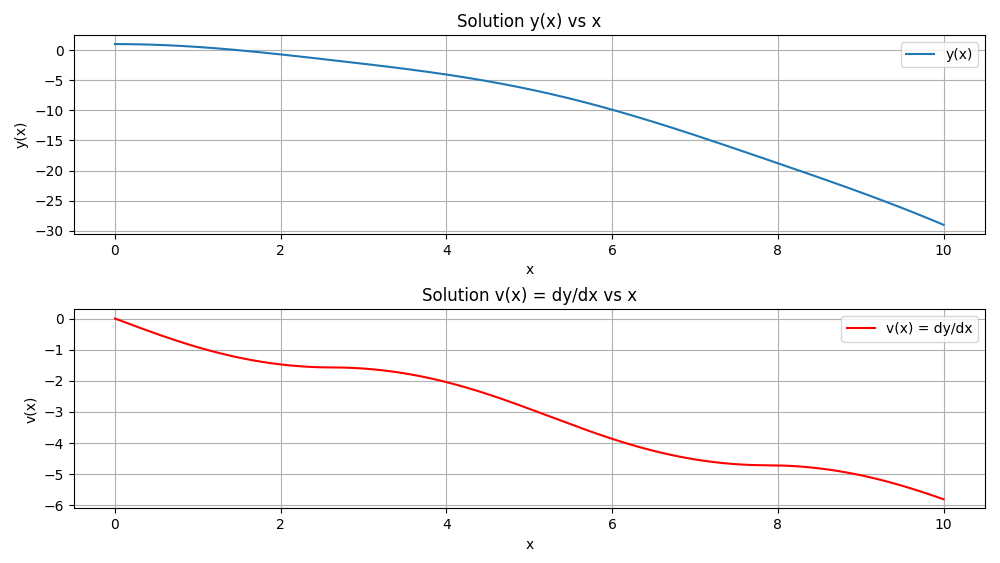
\includegraphics[width=\columnwidth]{fig/Figure_1.png}  
    \caption{Numerical result}
    \label{fig:results}
\end{figure}
\end{frame}

\begin{frame}{Conclusion}
\begin{block}{Summary}
\begin{itemize}
    \item Euler’s method is simple but prone to instability and inaccuracy, especially for nonlinear systems.
    \item The Runge-Kutta method offers higher accuracy and stability, making it the preferred choice for this kind of ODE.
    \item The RK4 method provides better results with fewer steps due to its higher-order accuracy.
\end{itemize}
\end{block}
\end{frame}

\end{document}

